\chapter{Acoplamientos Magnéticos y Transformadores}\label{chap.transformadores}

\section{Acoplamientos magnéticos}
\label{sec:acoplamientos}

\subsection{Fundamentos Físicos}
\label{sec:fisica-bobina}

Según la ley de Ampere, una corriente eléctrica circulando por un conductor crea un campo magnético en torno al conductor (\emph{regla de la mano derecha}).

\begin{center}
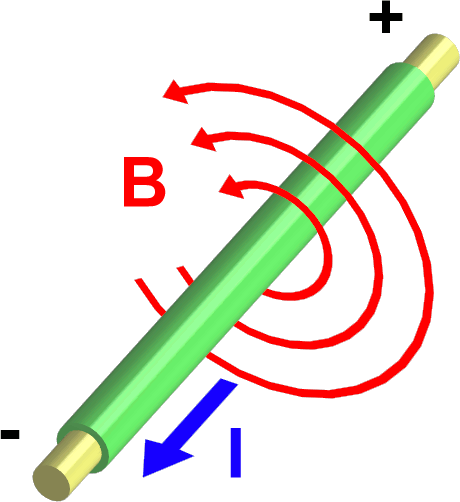
\includegraphics[height=0.2\textheight]{../figs/Electromagnetism.png}
\end{center}

Por otra parte, la ley de Faraday establece que cuando un \emph{campo magnético variable}, $\vec{B}$, atraviesa una espira \emph{estática} aparece una \emph{tensión inducida} \emph{proporcional al flujo} y opuesta a su variación.

\[
u(t) = \frac{\mathrm{d}\phi}{\mathrm{d}t} 
\]
donde $\phi$ es el flujo magnético o cantidad de líneas de fuerza magnética que atraviesan una superficie:

\[
\phi = \vec{B} \cdot \vec{A} \ [\mathrm{Wb}]
\]

\begin{figure}
  \centering
  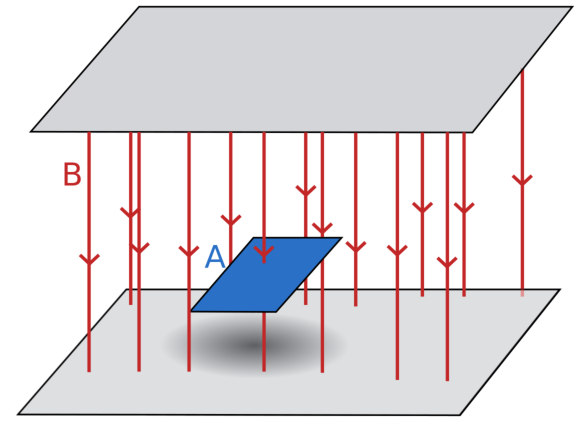
\includegraphics[height=0.2\textheight]{../figs/flujo_magnetico.pdf}
  \caption{Flujo magnético atravesando una superficie.}
  \label{fig:flujo-magnetico}
\end{figure}

Combinando ambas leyes podemos comprender el funcionamiento de la bobina. Una bobina es un arrollamiento de un conductor (\emph{conjunto de $N$ espiras conectadas en serie}) alrededor de un material ferromagnético:
\begin{itemize}
\item Al circular corriente se produce un campo magnético (\emph{ley de Ampere}).
\item Este campo magnético atraviesa la propia bobina y produce una tensión (auto)inducida (\emph{ley de Faraday}).
\end{itemize}

Por tanto, en una bobina de $N$ espiras la tensión autoinducida es:
\[
u(t) = N \cdot \frac{\mathrm{d}\phi(t)}{\mathrm{d} t}
\]

\begin{center}
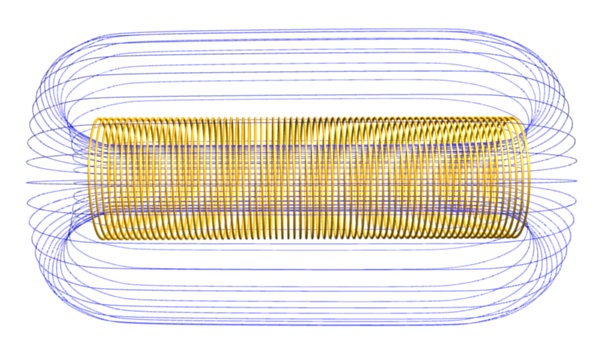
\includegraphics[height=0.2\textheight]{../figs/Solenoide.jpg}
\end{center}

Teniendo en cuenta que en circuito magnético lineal el flujo magnético es proporcional a la corriente:
\[
  \phi(t) = A \cdot i(t) \rightarrow   \frac{\mathrm{d}\phi(t)}{\mathrm{d} i(t)} = \frac{\phi(t)}{i(t)}
\]
podemos obtener la tensión inducida en función de la corriente eléctrica:
\[
u(t) = N \cdot \frac{\mathrm{d}\phi(t)}{\mathrm{d} i(t)} \cdot  \frac{\mathrm{d}i(t)}{\mathrm{d} t} \rightarrow u(t) = N \cdot \frac{\phi(t)}{i(t)} \cdot \frac{\mathrm{d}i(t)}{\mathrm{d} t}
\]
y, en consecuencia, determinamos el coeficiente de autoinductancia, $L \quad [H]$:
\[
  \boxed{L = N \cdot \frac{\phi(t)}{i(t)}}
\]
y la ecuación de la bobina que utilizamos en los circuitos:
\begin{equation}
  \label{eq:bobina-VI}
  \boxed{u(t) = L \cdot \frac{\mathrm{d}i(t)}{\mathrm{d} t}}
\end{equation}

\begin{center}
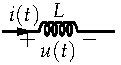
\includegraphics[height=0.1\textheight]{../figs/Bobina.pdf}
\end{center}

\subsection{Acoplamiento magnético}
\label{sec:acoplamiento}

Cuando dos bobinas comparten el núcleo ferromagnético, el flujo magnético producido por cada una de ellas atraviesa a la otra bobina, lo que se conoce como acoplamiento magnético (figura \ref{fig:acoplamiento}).

\begin{figure}
  \centering
  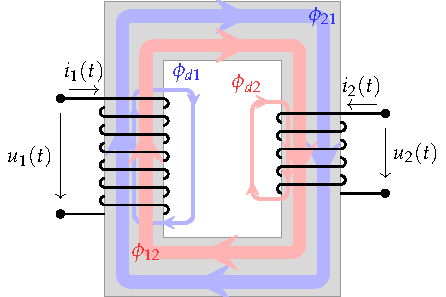
\includegraphics[height=0.2\textheight]{../figs/acoplamientoTikz.pdf}
    \caption{Acoplamiento magnético de dos bobinas. Definición de flujos.}
  \label{fig:acoplamiento}
\end{figure}

En la figura \ref{fig:acoplamiento} se indican los siguientes flujos:
\begin{itemize}
\item   $\phi_{ii}$: flujo producido por la bobina $i$
\item   $\phi_{ij}$: flujo recibido en bobina $i$ producido por bobina $j$
\item   $\phi_{i}$: flujo total que atraviesa la bobina $i$
\item   $\phi_{di}$: flujo de dispersión de la bobina $i$, o flujo que escapa del núcleo y no contribuye al acoplamiento.
\end{itemize}

Estos flujos cumplen las siguientes relaciones:
\begin{align*}
  \phi_{11} &= \phi_{d1} + \phi_{21}\\
  \phi_{1} &= \phi_{11} + \phi_{12}\\
  \phi_{22} &= \phi_{d2} + \phi_{12}\\
  \phi_{2} &= \phi_{22} + \phi_{21}
\end{align*}

La ratio entre el flujo que recibe una bobina y el flujo producido por la bobina emisora se cuantifica con los coeficientes de acoplamiento $k_i$ :
\begin{align}
  \label{eq:coefs-acoplamiento}
  k_1 = \frac{\phi_{21}}{\phi_{11}} = 1 - \frac{\phi_{d1}}{\phi_{11}} \leq 1
  k_2 = \frac{\phi_{12}}{\phi_{22}} = 1 - \frac{\phi_{d2}}{\phi_{22}} \leq 1
\end{align}
Cuando el acoplamiento entre las dos bobinas es perfecto, los flujos de dispersión son nulos y, por tanto:
\[\left.
\begin{array}{cc}
  \phi_{d1} = 0 \rightarrow   \phi_{11} = \phi_{21}\\
  \phi_{d2} = 0 \rightarrow \phi_{22} = \phi_{12} 
  \end{array} \right\} \rightarrow k = 1
\]

A partir de los flujos que recorren el núcleo obtenemos las tensiones inducidas en la bobina 1:
\begin{align*}
  u_1(t) = &N_1 \frac{\mathrm{d}\phi_1}{\mathrm{d}t} = \\
  &N_1 \frac{\mathrm{d}\phi_{11}}{\mathrm{d}t} + N_1 \frac{\mathrm{d}\phi_{12}}{\mathrm{d}t}
\end{align*}
y en la bobina 2:
\begin{align*}
  u_2(t) = &N_2 \frac{\mathrm{d}\phi_2}{\mathrm{d}t} = \\
  &N_2 \frac{\mathrm{d}\phi_{22}}{\mathrm{d}t} + N_2 \frac{\mathrm{d}\phi_{21}}{\mathrm{d}t}
\end{align*}

En estas ecuaciones podemos identificar los términos debidos a la autoinducción, con sus dos coeficientes de autoinducción:
\begin{align}
  \label{eq:acoplamiento-autoinduccion}
  L_1 &= N_1 \frac{\phi_{11}}{i_1}\\
  L_2 &= N_2 \frac{\phi_{22}}{i_2}
\end{align}
y los términos de inducción mutua, con los que podemos definir los coeficientes de inducción mutua, $M_{12}$ y $M_{21}$:
\begin{align}
  \label{eq:coef-induccion-mutua}
  M_{12} &= N_1 \frac{\phi_{12}}{i_2}\\
  M_{21} &= N_2 \frac{\phi_{21}}{i_1}
\end{align}

Los coeficientes de acoplamiento y los coeficientes de inducción mutua son iguales cuando el circuito magnético es lineal:
  \begin{align*}
  M_{12} = M_{21} &= M\\
  k_1 = k_2 &= k    
  \end{align*}
  Esta condición nos permite relacionar los coeficientes de autoinducción con el coeficiente de inducción mutua:
  \begin{equation}
    \label{eq:L-M}
    \boxed{M = k \sqrt{L_1 \cdot L_2}} \qquad  k \leq 1
  \end{equation}

\subsection{Representación Circuital}
\label{sec:org1754ad3}
Para representar un acoplamiento magnético en un circuito eléctrico se
emplea la convención del punto, señalando con un punto los terminales
de las bobinas por los que hay que introducir corrientes que producen
flujos del mismo sentido. Una corriente que entra por un terminal con
punto induce una tensión positiva en el otro terminal con punto.

En la siguiente figura, las dos bobinas están arrolladas de forma que introduciendo corrientes por los terminales superiores se obtienen flujos que circulan en el mismo sentido:
\begin{center}
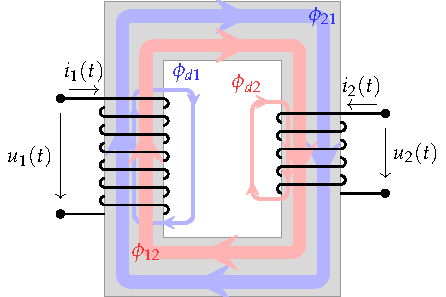
\includegraphics[height=0.2\textheight]{../figs/acoplamientoTikz.pdf}
\end{center}

\begin{center}
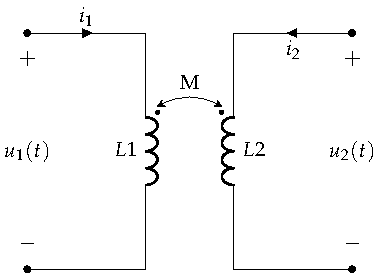
\includegraphics[height=0.2\textheight]{../figs/acoplamiento_circuito.pdf}
\end{center}

Las ecuaciones circuitales de este acoplamiento son:
\begin{align*}
  u_1(t) &= L_1 \frac{\mathrm{d}i_1(t)}{\mathrm{d}t} + M \frac{\mathrm{d}i_2(t)}{\mathrm{d}t}\\
  u_2(t) &= M \frac{\mathrm{d}i_1(t)}{\mathrm{d}t} + L_2 \frac{\mathrm{d}i_2(t)}{\mathrm{d}t}
\end{align*}

Por el contrario, la siguiente figura representa un acoplamiento en el que las bobinas están arrolladas de forma que los flujos tienen sentidos contrapuestos si se introduce corriente por los terminales superiores. 

\begin{center}
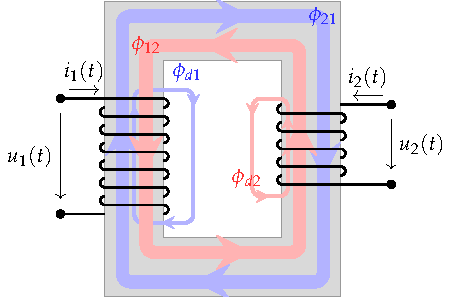
\includegraphics[height=0.2\textheight]{../figs/acoplamientoTikz_opuesto.pdf}
\end{center}
\begin{center}
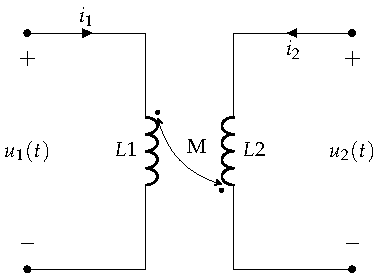
\includegraphics[height=0.2\textheight]{../figs/acoplamiento_circuito_opuesto.pdf}
\end{center}

Las ecuaciones circuitales de este acoplamiento son:

\begin{align*}
  u_1(t) &= L_1 \frac{\mathrm{d}i_1(t)}{\mathrm{d}t} - M \frac{\mathrm{d}i_2(t)}{\mathrm{d}t}\\
  u_2(t) &= - M \frac{\mathrm{d}i_1(t)}{\mathrm{d}t} + L_2 \frac{\mathrm{d}i_2(t)}{\mathrm{d}t}
\end{align*}

Las ecuaciones anteriores están expresadas en el dominio del tiempo. Cuando las bobinas están alimentadas por corriente alterna sinusoidal, podemos expresar las ecuaciones con fasores, ya sea para flujos en el mismo sentido:
\begin{align*}
  \overline{U}_1 &= j \omega L_1 \overline{I}_1 + j \omega M \overline{I}_2\\
  \overline{U}_2 &= j \omega M \overline{I}_1 + j \omega L_2 \overline{I}_2
\end{align*}
o para flujos contrapuestos:
\begin{align*}
  \overline{U}_1 &= j \omega L_1 \overline{I}_1 - j \omega M \overline{I}_2\\
  \overline{U}_2 &= - j \omega M \overline{I}_1 + j \omega L_2 \overline{I}_2
\end{align*}


Como ejemplo, calculemos la bobina equivalente de dos bobinas conectadas en serie. Cuando las bobinas están acopladas con flujos en el mismo sentido (figura \ref{fig:bobinas-serie-mismo-sentido}), las ecuaciones son:

\begin{figure}
  \centering
  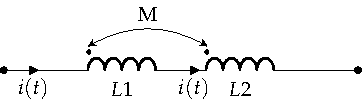
\includegraphics[height=0.1\textheight]{../figs/bobinas_serie.pdf}
  \caption{Dos bobinas conectadas en serie con acoplamiento magnético con flujos en el mismo sentido.}
  \label{fig:bobinas-serie-mismo-sentido}
\end{figure}

  \begin{align*}
    \overline{U}_1 &= (j \omega L_1 + j \omega M) \overline{I}\\
    \overline{U}_2 &= (j \omega L_2 + j \omega M) \overline{I}\\
    \overline{U} &= \overline{U}_1 + \overline{U}_2 
  \end{align*}
que permiten obtener la equivalencia de la ecuación \ref{eq:bobinas-serie-coincidente}:
\begin{equation}
  \label{eq:bobinas-serie-mismo-sentido}
  L = L_1 + L_2 + 2M
\end{equation}

Sin embargo, si las bobinas están acopladas con flujos contrapuestos (figura \ref{fig:bobinas-serie-flujo-contrapuesto}), las ecuaciones son:
\begin{figure}
  \centering
  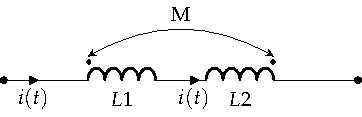
\includegraphics[height=0.1\textheight]{../figs/bobinas_serie_opuesto.pdf}
  \caption{Dos bobinas conectadas en serie con acoplamiento magnético  con flujos contrapuestos.}
  \label{fig:bobinas-serie-flujo-contrapuesto}
\end{figure}

\begin{align*}
  \overline{U}_1 &= (j \omega L_1 - j \omega M) \overline{I}\\
  \overline{U}_2 &= (j \omega L_2 - j \omega M) \overline{I}\\
  \overline{U} &= \overline{U}_1 + \overline{U}_2 
\end{align*}
de forma que la inductancia equivalente es ahora:
\begin{equation}
  \label{eq:bobinas-serie-contrapuesto}
  L = L_1 + L_2 - 2M
\end{equation}

\section{Transformadores}
\label{sec:transformadores}

Un transformador es una máquina eléctrica compuesta por dos o más devanados arrollados sobre un núcleo ferromagnético sin conexión eléctrica entre los devanados (figura \ref{fig:acoplamiento}), de forma que la transmisión de energía se realiza únicamente mediante el acoplamiento magnético.

\subsection{Transformador Real}
\label{sec:transformador-real}

La figura \ref{fig:trafo-real} es la representación circuital simplificada de un transformador real, es decir, un transformador que tiene pérdidas resistivas en las bobinas y cuyo acoplamiento magnético no es perfecto ($k < 1$).

\begin{figure}
  \centering
  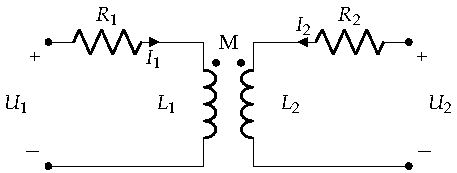
\includegraphics[height=0.2\textheight]{../figs/Trafo_Real.pdf}
  \caption{Representación circuital de un transformador real}
  \label{fig:trafo-real}
\end{figure}
Las ecuaciones de este transformador son:
\begin{align}
  \label{eq:trafo-real}
  \overline{U}_1 &= (R_1 + j \omega L_1) \cdot \overline{I}_1 + j \omega M \cdot\overline{I}_2\\
  \overline{U}_2 &= j \omega M \cdot \overline{I}_1 + (R_2 + j \omega L_2) \cdot \overline{I}_2
\end{align}

En general, los terminales de la izquierda ($U_1$) se denominan como primario, y los terminales de la derecha ($U_2$) como secundario.

Supongamos que conectamos una impedancia en el secundario de este transformador. Para calcular la impedancia que se ve desde el primario debemos calcular la relación $\overline{U}_1/\overline{I}_1$ a partir de las ecuaciones \ref{eq:trafo-real} y de la
ecuación de la impedancia:

\begin{equation*}
  \overline{U}_2 = - \overline{I}_2 \cdot \overline{Z}_L
\end{equation*}

\begin{figure}
  \centering
  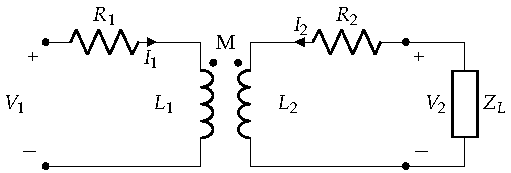
\includegraphics[height=0.2\textheight]{../figs/Trafo_Real_ImpSec.pdf}
  \caption{Impedancia conectada en el secundario de un transformador real.}
  \label{fig:trafo-real-impedancia-secundario}
\end{figure}


Combinando la ecuación del secundario con la ecuación de la carga obtenemos la corriente en el secundario:
\[
  \overline{I}_2  = - \frac{j \omega M}{(R_2 + j \omega L_2) + \overline{Z}_L} \cdot \overline{I}_1
\]
que podemos insertar en la ecuación del primario para obtener la impedancia de entrada:

\begin{equation}
  \label{eq:trafo-real-impedancia-entrada}
  \overline{Z}_{in}  = \frac{\overline{U}_1}{\overline{I}_1} =  (R_1 + j \omega L_1) + \frac{\omega^2 M^2}{(R_2 + j \omega L_2) + \overline{Z}_L} = \boxed{\overline{Z}_1 + \frac{\omega^2 M^2}{\overline{Z}_2 + \overline{Z}_L}}
\end{equation}
Podemos interpretar este resultado como la conexión serie de la impedancia de primario con una impedancia transformada, obtenida a partir de la conexión serie de la impedancia de secundario y la impedancia de carga.

Calculemos ahora el equivalente de Thévenin desde secundario de una fuente real conectada en el primario (figura \ref{fig:trafo-real-fuente-primario}).

\begin{figure}
  \centering
  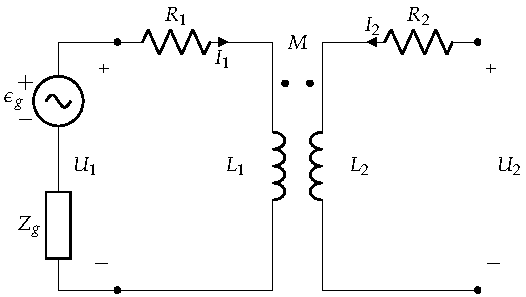
\includegraphics[height=0.2\textheight]{../figs/Trafo_Real_FuentePrimario.pdf}
  \caption{Fuente real conectada en el primario de un transformador real.}
  \label{fig:trafo-real-fuente-primario}
\end{figure}

La ecuación del generador es:
\[
  \overline{U}_1 = \overline{\epsilon}_g - \overline{I}_1 \cdot \overline{Z}_g
\]
mientras que las ecuaciones del transformador se simplifican al tener en cuenta que $\overline{I}_2 = 0$:
\begin{align*}
  \overline{U}_1 &= (R_1 + j \omega L_1) \cdot \overline{I}_1\\
  \overline{U}_2 &= j \omega M \cdot \overline{I}_1
\end{align*}
Despejamos la corriente de primario $I_1$:
\[
  \overline{I}_1 = \frac{\overline{\epsilon_g}}{\overline{Z}_1 + \overline{Z}_g}
\]
y la utilizamos en la ecuación del secundario para obtener la tensión de Thévenin:

\begin{equation}
  \label{eq:trafo-real-tension-thevenin}
  \overline{U}_2 = \boxed{\overline{\epsilon}_{th} = \frac{j\omega M}{\overline{Z}_1 + \overline{Z}_g} \cdot \overline{\epsilon}_g}
\end{equation}
Este resultado recuerda a la expresión de un divisor de tensión, aunque el numerador está transformado respecto a la expresión original.

Para calcular la impedancia de Thévenin apagamos la fuente $\epsilon_g$ y conectamos una fuente de prueba en secundario (figura \ref{fig:trafo-real-impedancia-thevenin}). 
\begin{figure}
  \centering
  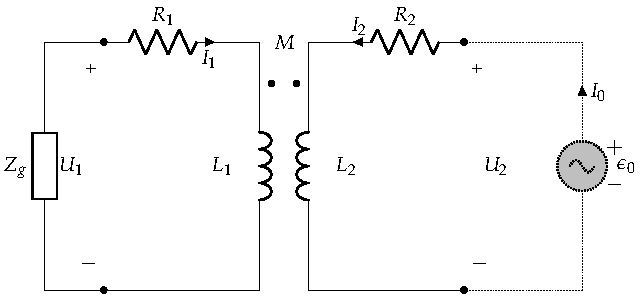
\includegraphics[height=.2\textheight]{../figs/Trafo_Real_ImpedanciaPrimario.pdf}
    \caption{Cálculo de la impedancia de Thévenin de una fuente conectada en primario.}
  \label{fig:trafo-real-impedancia-thevenin}
\end{figure}
Con esta conexión, las ecuaciones del transformador son:
\begin{align*}
  \overline{U}_1 &= (R_1 + j \omega L_1) \cdot \overline{I}_1 + j \omega M \cdot\overline{I}_0\\
  \overline{\epsilon}_0 &= j \omega M \cdot \overline{I}_1 + (R_2 + j \omega L_2) \cdot \overline{I}_0
\end{align*}
y la ecuación de la impedancia:
\[
  \overline{U}_1 = - \overline{Z}_g \cdot \overline{I}_1
\]
Combinando estas ecuaciones obtenemos la impedancia de Thévenin:

\begin{equation}
  \label{eq:trafo-real-impedancia-thevenin}
  \boxed{\overline{Z}_{th} = \frac{\overline{\epsilon}_0}{\overline{I}_0} = \overline{Z}_2 + \frac{\omega^2 M^2}{\overline{Z}_1 + \overline{Z}_g}}
\end{equation}
Esta expresión, al igual que la ecuación \ref{eq:trafo-real-impedancia-entrada}, se asemeja a la conexión serie de la impedancia de secundario con una impedancia transformada obtenida a partir de la impedancia de primario y del generador.

\subsection{Transformador Perfecto}
\label{sec:trafo-perfecto}

Un transformador perfecto (figura \ref{fig:trafo-perfecto}) es aquel en el que las pérdidas resistivas son despreciables.
\[
  R_1 = R_2 = 0
\]
y el acoplamiento es perfecto.
\[
  k = 1
\rightarrow 
\left\{
\begin{array}{cc}
  \phi_{12} &= \phi_{22}\\
  \phi_{21} &= \phi_{11}\\
\end{array} \right.
\]

\begin{figure}
  \centering
  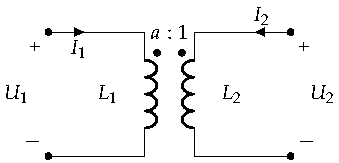
\includegraphics[height=0.2\textheight]{../figs/Trafo_Perfecto.pdf}
  \caption{Representación circuital de un transformador perfecto.}
  \label{fig:trafo-perfecto}
\end{figure}

Las ecuaciones de este transformador son:
\begin{align*}
  \overline{U}_1 &= j \omega L_1 \cdot \overline{I}_1 + j \omega M \cdot \overline{I}_2\\
  \overline{U}_2 &= j \omega M \cdot \overline{I}_1 + j \omega L_2 \cdot \overline{I}_2
\end{align*}

Teniendo en cuenta que $k = 1$, a partir de las ecuaciones de $M_{12} = M_{21} = M$:
\[
  N_1 \frac{\phi_{12}}{i_2} = N_2 \frac{\phi_{21}}{i_1}
\]
podemos escribir:
\[  
  N_1 \frac{\phi_{22}}{i_2} = N_2 \frac{\phi_{11}}{i_1}
\]
Además, con las definiciones de $L_1$ y $L_2$:
\[
  N_1 \frac{L_2}{N_2} = N_2 \frac{L_1}{N_1}
\]
obtenemos la relación de transformación de un transformador perfecto:
\begin{equation}
  \label{eq:trafo-perfecto-a}
  \boxed{\frac{L_1}{L_2} = \left(\frac{N_1}{N_2}\right)^2 = a^2}
\end{equation}


Con esta relación de transformación podemos simplificar las ecuaciones del transformador. En primer lugar dividimos las ecuaciones:
\[
  \frac{\overline{U}_1}{\overline{U}_2} = \frac{j \omega L_1 \cdot \overline{I}_1 + j \omega M \cdot \overline{I}_2}{j \omega M \cdot \overline{I}_1 + j \omega L_2 \cdot \overline{I}_2}
\]
y empleamos la relación de transformación:
\[
  \frac{L_1}{L_2} = a^2
  \rightarrow
  \left\{
  \begin{array}{ll}
    L_1 &= a^2 \cdot L_2\\
    M &= a \cdot L_2\\
  \end{array}\right.
\]
para escribir:
\[
  \frac{\overline{U}_1}{\overline{U}_2} = \frac{a^2 L_2 \cdot \overline{I}_1 + a L_2 \cdot \overline{I}_2}{a L_2 \cdot \overline{I}_1 + L_2 \cdot \overline{I}_2}
\]
que, después de simplificar, conduce a la relación entre tensiones de un transformador perfecto:
\begin{equation}
  \label{eq:trafo-perfecto-tensiones}
  \boxed{\frac{\overline{U}_1}{\overline{U}_2} = a = \frac{N_1}{N_2}}
\end{equation}

Estas relaciones nos permiten simplificar los resultados obtenidos con el transformador real. En primer lugar, la impedancia de entrada en un transformador real con $R_1 = R_2 = 0$ es:

\[
  \overline{Z}_{in} = j\omega L_1 + \frac{\omega^2 M^2}{j\omega L_2 + \overline{Z}_L}
\]

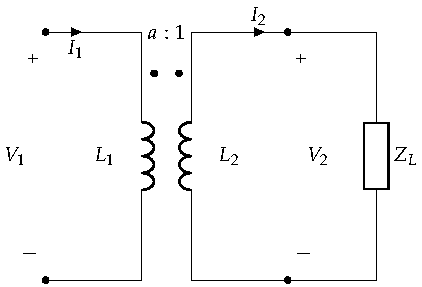
\includegraphics[height=0.2\textheight]{../figs/TrafoPerfecto_ImpedanciaSecundario.pdf}


A continuación, teniendo en cuenta la relación entre $L_1$, $L_2$ y $M$:
\[
  \overline{Z}_{in} = j\omega L_1 + \frac{\omega^2 M^2}{j\omega L_2 + \overline{Z}_L} = \frac{j\omega L_1 \overline{Z}_L}{j\omega L_2 + \overline{Z}_L}
\]
y, finalmente, incorporando la relación de transformación:
\begin{equation}
  \label{eq:trafo-perfecto-impedancia-entrada}
  \overline{Z}_{in} =  a^2 \cdot \frac{j \omega L_2 \cdot \overline{Z}_L}{j\omega L_2 + \overline{Z}_L} =  \frac{j \omega L_1 \cdot a^2 \cdot \overline{Z}_L}{j\omega L_1 + a^2 \cdot \overline{Z}_L}
\end{equation}
Esta expresión se puede interpretar como un factor de escala aplicado a una conexión en paralelo entre la inductancia de secundario y la impedancia de carga, o como una conexión en paralelo entre la inductancia de primario y la impedancia de carga con un factor de escala.

De forma equivalente, el equivalente de Thévenin de una fuente real conectada en primario es:

\[
  \overline{\epsilon}_{th} = \overline{U}_2 = \frac{j\omega M}{j\omega L_1 + \overline{Z}_g} \cdot \overline{\epsilon}_g
\]

\begin{center}
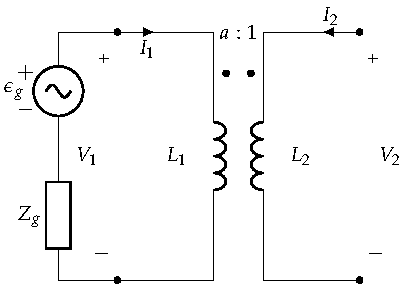
\includegraphics[height=0.2\textheight]{../figs/Trafo_Perfecto_FuentePrimario.pdf}
\end{center}

Teniendo en cuenta que $M = L_1/a$:
\[
  \overline{\epsilon}_{th} = \frac{1}{a} \cdot \left(\frac{j\omega L_1}{j\omega L_1 + \overline{Z}_g}\right) \cdot \overline{\epsilon}_g
\]
Esta expresión corresponde a un divisor de tensión entre la impedancia del generador y la inductancia del primario, aplicando previamente un factor de escala.

Por otra parte, la impedancia de Thévenin es:
\[
  \overline{Z}_{th} = j\omega L_2 + \frac{\omega^2 M^2}{j\omega L_1 + \overline{Z}_g}
\]
Aplicando las relaciones $L_2 = L_1/a^2$ y $M = L_1/a$ obtenemos:
\begin{equation}
  \label{eq:trafo-perfecto-impedancia-thevenin}
  \overline{Z}_{th} = \frac{1}{a^2} \cdot \frac{j \omega L_1 \cdot \overline{Z}_g}{j\omega L_1 + \overline{Z}_g}
\end{equation}
Este resultado se puede interpretar como una impedancia equivalente de una conexión en paralelo entre la inductancia de primario y la impedancia del generador, aplicando previamente un factor de escala.



% \section{Transformador Ideal}
% \label{sec:orgafd2d9c}
% \begin{frame}[label={sec:org4f54a79}]{Definición}
% \begin{center}
% 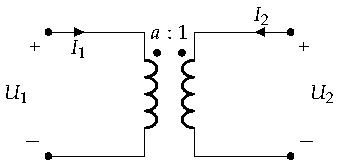
\includegraphics[height=0.35\textheight]{../figs/Trafo_Ideal.pdf}
% \end{center}

% Las pérdidas resistivas son despreciables.
% \[
%   R_1 = R_2 = 0
% \]

% El acoplamiento es perfecto.
% \[
%   k = 1
% \]

% Las bobinas tienen un número muy elevado de espiras.
% \begin{align*}
%   N_1 &\to \infty\\
%   N_2 &\to \infty
% \end{align*}
% \end{frame}
% \begin{frame}[label={sec:org0c06567}]{El flujo en cada bobina es nulo}
% Para que las tensiones inducidas sean finitas\ldots{} 

% \begin{align*}
%   \overline{U}_1 &= N_1 \overline{\phi}_1\\ 
%   \overline{U}_2 &= N_2 \overline{\phi}_2
% \end{align*}
% \ldots{}los flujos (fasoriales) que los atraviesan deben ser nulos.
% \begin{align*}
%   \overline{\phi}_1 &\to 0\\
%   \overline{\phi}_2 &\to 0\\
% \end{align*}
% Siendo:
% \begin{align*}
%   \overline{\phi}_1 &= \overline{\phi}_{11} + \overline{\phi}_{12}\\
%   \overline{\phi}_2 &= \overline{\phi}_{22} + \overline{\phi}_{21}
% \end{align*}
% \end{frame}
% \begin{frame}[label={sec:org075f3f1}]{El flujo mutuo es nulo}
% Teniendo en cuenta que el acoplamiento es perfecto, $k = 1$:
% \[
%   \left.
%     \begin{array}{ll}
%       \phi_{12} &= \phi_{22}\\
%       \phi_{21} &= \phi_{11}\\
%     \end{array} \right\} 
%   \rightarrow
%   \left\{
%     \begin{array}{ll}
%       0 &= \overline{\phi}_{21} + \overline{\phi}_{12}\\
%       0 &= \overline{\phi}_{12} + \overline{\phi}_{21}\\
%     \end{array}\right.
% \]

% O también:

% \[
%   \boxed{\overline{\phi}_{11} + \overline{\phi}_{22} = 0}
% \]
% \end{frame}
% \begin{frame}[label={sec:orgb9f5ba1}]{Relación de Transformación}
% Hemos obtenido:
% \[
%   \overline{\phi}_{11} + \overline{\phi}_{22} = 0
% \]

% Con las definiciones de $L_1$, $L_2$:
% \[
%   L_1 = N_1 \frac{\phi_{11}}{I_1}; \quad L_2 = N_2 \frac{\phi_{22}}{I_2}
% \]
% Podemos escribir:
% \[
%   \frac{L_1 \overline{I}_1}{N_1} + \frac{L_2 \overline{I}_2}{N_2} = 0
% \]
% Y con la relación entre ambas obtenemos
% \[
%   L_1 = L_2 \cdot \left(\frac{N_1}{N_2}\right)^2
%   \rightarrow
%   \frac{N_1L_2 \overline{I}_1}{N^2_2} + \frac{L_2 \overline{I}_2}{N_2} = 0
%   \rightarrow
%   \boxed{\frac{\overline{I}_1}{\overline{I}_2} = \mp \frac{1}{a} = \mp \frac{N_2}{N_1}}
% \]
% \end{frame}
% \begin{frame}[label={sec:org6b09b30}]{Un transformador ideal no consume potencia}
% \[
%   \overline{S}_1 = \overline{U}_1 \cdot \overline{I}_1^*
% \]

% \[
%   \overline{S}_2 = \overline{U}_2 \cdot \overline{I}_2^* 
% \]

% \[
%   \overline{U}_2 \cdot \overline{I}_2^* = \frac{1}{a} \cdot \overline{U}_1 \cdot a \cdot \overline{I}_1^* = \overline{S}_1
% \]

% \[
%   \boxed{\overline{S}_1 = \overline{S}_2}
%   \quad
%   \boxed{P_1 = P_2}
%   \quad
%   \boxed{Q_1 = Q_2}
% \]
% \end{frame}
% \section{Transferencia de Circuitos}
% \label{sec:orga4512fa}
% \begin{frame}[label={sec:orgd972ca8}]{Fuente de Tensión de Secundario a Primario}
% \begin{center}
% 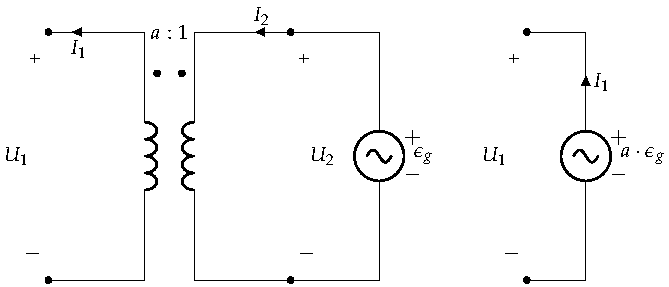
\includegraphics[height=.2\textheight]{../figs/TrafoIdeal_VSec.pdf}
% \end{center}

% \[
%   \overline{U}_1 = a \cdot \overline{U}_2 \rightarrow \boxed{\overline{\epsilon}_{g1} = a \cdot \overline{\epsilon}_g}
% \]
% \end{frame}
% \begin{frame}[label={sec:org7862583}]{Fuente de Tensión de Primario a Secundario}
% \begin{center}
% 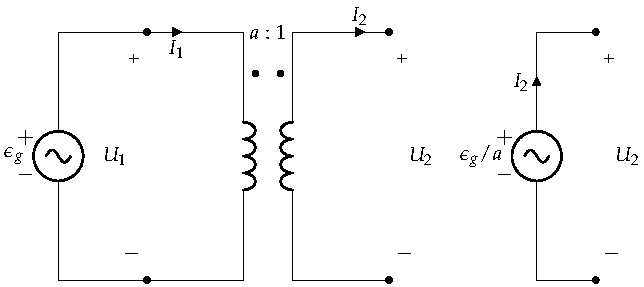
\includegraphics[height=.2\textheight]{../figs/TrafoIdeal_VPrim.pdf}
% \end{center}

% \[
%   \overline{U}_2 = \overline{U}_1 / a \rightarrow \boxed{\overline{\epsilon}_{g2} = \overline{\epsilon}_g / a}
% \]
% \end{frame}
% \begin{frame}[label={sec:org42d6d3c}]{Fuente de Corriente de Secundario a Primario}
% \begin{center}
% 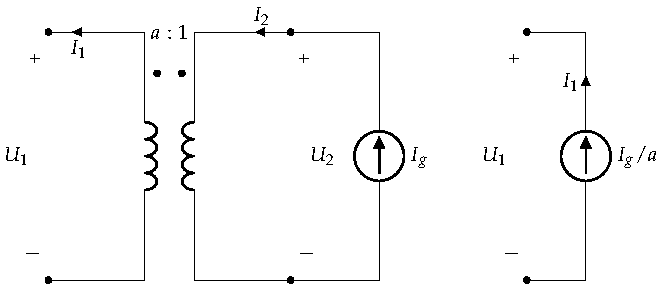
\includegraphics[height=.2\textheight]{../figs/TrafoIdeal_ISec.pdf}
% \end{center}

% \[
%   \overline{I}_1 = \overline{I}_2 / a \rightarrow \boxed{\overline{I}_{g1} = \overline{I}_g / a} 
% \]
% \end{frame}
% \begin{frame}[label={sec:org286163b}]{Fuente de Corriente de Primario a Secundario}
% \begin{center}
% 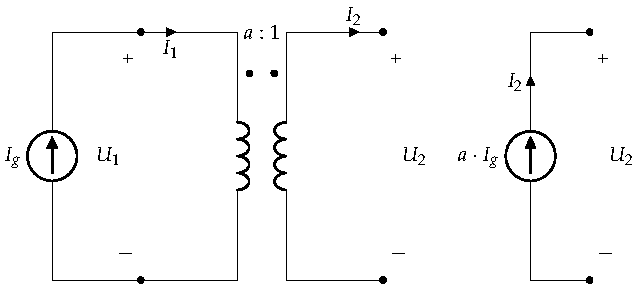
\includegraphics[height=.2\textheight]{../figs/TrafoIdeal_IPrim.pdf}
% \end{center}
% \[
%   \overline{I}_2 = a \cdot \overline{I}_1 \rightarrow \boxed{\overline{I}_{g2} = a \cdot \overline{I}_g}
% \]
% \end{frame}
% \begin{frame}[label={sec:orgfcbf5df}]{Impedancia de Secundario a Primario}
% \begin{center}
% 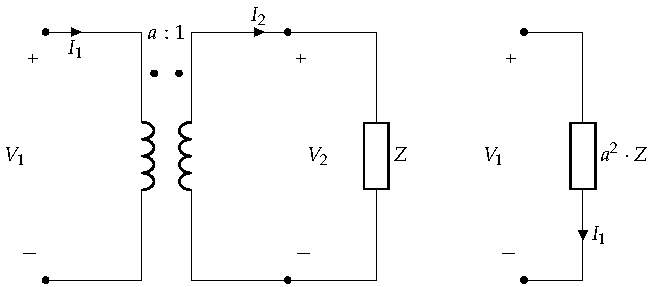
\includegraphics[height=.2\textheight]{../figs/TrafoIdeal_ZSec.pdf}
% \end{center}
% \[
%   \left.
%     \begin{array}{ll}
%     \overline{U}_1 &= a \cdot \overline{U}_2\\
%     \overline{I}_1 &= \overline{I}_2 / a\\
%   \end{array}\right\}
%    \rightarrow \boxed{\overline{Z}_1 = \frac{\overline{U}_1}{\overline{I}_1} = a^2 \cdot \overline{Z}} 
% \]
% \end{frame}
% \begin{frame}[label={sec:org8fb9ac2}]{Impedancia de Primario a Secundario}
% \begin{center}
% 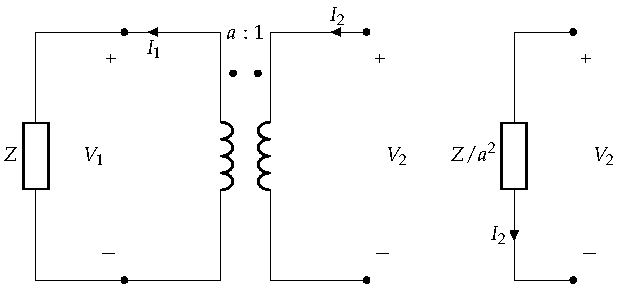
\includegraphics[height=.2\textheight]{../figs/TrafoIdeal_ZPrim.pdf}
% \end{center}
% \[
%   \left.
%     \begin{array}{ll}
%     \overline{U}_2 &= \overline{U}_1 /a\\
%     \overline{I}_2 &= a \cdot \overline{I}_1\\
%   \end{array}\right\}
%    \rightarrow \boxed{\overline{Z}_2 = \frac{\overline{U}_2}{\overline{I}_2} = \overline{Z} / a^2} 
% \]
% \end{frame}
% \section{Transformador Perfecto vs. Transformador Ideal}
% \label{sec:org7f8bfa5}
% \begin{frame}[label={sec:org1a082ae}]{Recordatorio: impedancia de entrada de un T. Perfecto}
% \begin{center}
% 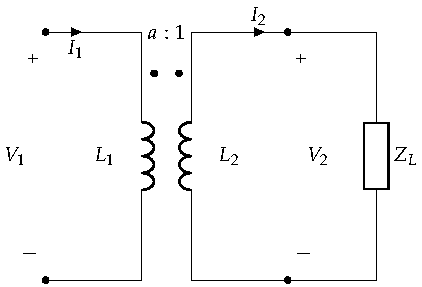
\includegraphics[height=0.45\textheight]{../figs/TrafoPerfecto_ImpedanciaSecundario.pdf}
% \end{center}

% \[
%   \boxed{\overline{Z}_{in} = \frac{j \omega L_1 \cdot (a^2 \overline{Z}_L)}{j\omega L_1 + (a^2 \cdot \overline{Z}_L)}}
% \]

% \[
%   \boxed{\overline{Z}_{in} = a^2 \cdot \frac{j \omega L_2 \cdot \overline{Z}_L}{j\omega L_2 + \overline{Z}_L}}
% \]
% \end{frame}
% \begin{frame}[label={sec:org3b521b8}]{Circuito equivalente con transformador ideal}
% \begin{columns}
% \begin{column}{0.5\columnwidth}
% \begin{center}
% 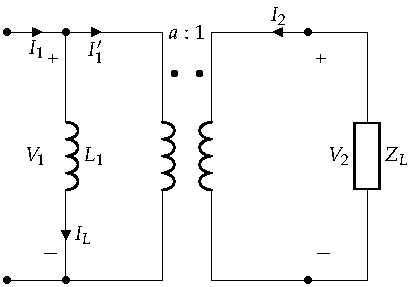
\includegraphics[height=.2\textheight]{../figs/TrafoPerfecto_Ideal.pdf}
% \end{center}

% \[
%   \boxed{\overline{Z}_{in} = \frac{j \omega L_1 \cdot (a^2 \overline{Z}_L)}{j\omega L_1 + (a^2 \cdot \overline{Z}_L)}}
% \]
% \end{column}
% \begin{column}{0.5\columnwidth}
% \begin{center}
% 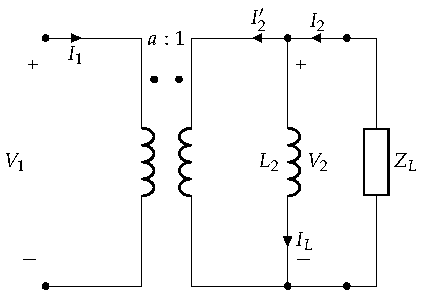
\includegraphics[height=.2\textheight]{../figs/TrafoPerfecto_Ideal2.pdf}
% \end{center}

% \[
%   \boxed{\overline{Z}_{in} = a^2 \cdot \frac{j \omega L_2 \cdot \overline{Z}_L}{j\omega L_2 + \overline{Z}_L}}
% \]
% \end{column}
% \end{columns}
% \end{frame}

% \begin{frame}[label={sec:org52c4dd9}]{Recordatorio: Equivalente de Thévenin}
% \begin{center}
% 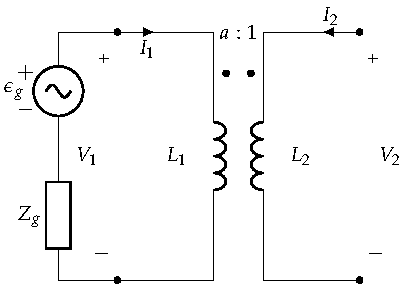
\includegraphics[height=0.5\textheight]{../figs/Trafo_Perfecto_FuentePrimario.pdf}
% \end{center}

% \[
%   \overline{Z}_{th} = \frac{1}{a^2} \cdot \frac{j \omega L_1 \cdot \overline{Z}_g}{j\omega L_1 + \overline{Z}_g}
% \]

% \[
%   \overline{\epsilon}_{th} = \frac{1}{a} \cdot \left(\frac{j\omega L_1}{j\omega L_1 + \overline{Z}_g}\right) \cdot \overline{\epsilon}_g
% \]
% \end{frame}

% \begin{frame}[label={sec:org102e193}]{Equivalente en primario con transformador ideal}
% \[
%   \overline{Z}_{th} = \frac{1}{a^2} \cdot \frac{j \omega L_1 \cdot \overline{Z}_g}{j\omega L_1 + \overline{Z}_g}
% \]

% \[
%   \overline{\epsilon}_{th} = \frac{1}{a} \cdot \left(\frac{j\omega L_1}{j\omega L_1 + \overline{Z}_g}\right) \cdot \overline{\epsilon}_g
% \]

% \begin{center}
% 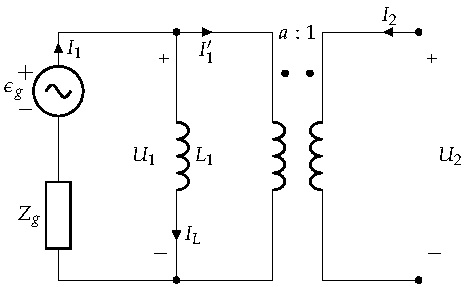
\includegraphics[height=0.5\textheight]{../figs/TrafoPerfecto_Ideal_FuentePrim.pdf}
% \end{center}
% \end{frame}
% \begin{frame}[label={sec:org16d210b}]{Equivalente en secundario con transformador ideal}
% \[
%   \overline{Z}_{th} = a^2 \cdot \frac{j \omega L_2 \cdot \overline{Z}_g}{j\omega L_2 + \overline{Z}_g}
% \]

% \[
%   \overline{\epsilon}_{th} = a \cdot \left(\frac{j\omega L_2}{j\omega L_2 + \overline{Z}_g}\right) \cdot \overline{\epsilon}_g
% \]

% \begin{center}
% 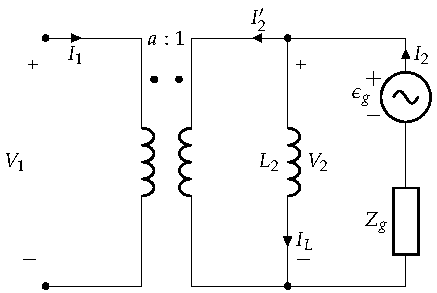
\includegraphics[height=0.5\textheight]{../figs/TrafoPerfecto_Ideal_FuenteSec.pdf}
% \end{center}
% \end{frame}
% \section{Transformador de Varios Devanados}
% \label{sec:org307d3d0}
% \begin{frame}[label={sec:org06465ee}]{Transformador Real de Varios Devanados}
% \begin{center}
% 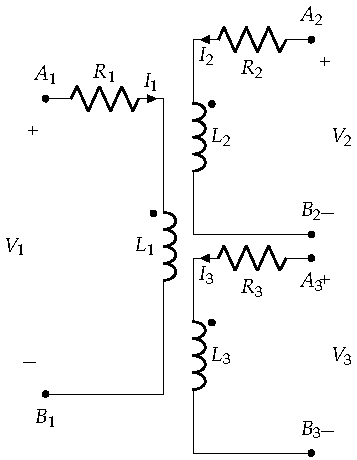
\includegraphics[height=0.9\textheight]{../figs/TrafoVariosDevanados.pdf}
% \end{center}
% \end{frame}

% \begin{frame}[label={sec:orgdccada5}]{Ecuaciones del Transformador Real}
% \begin{center}
% 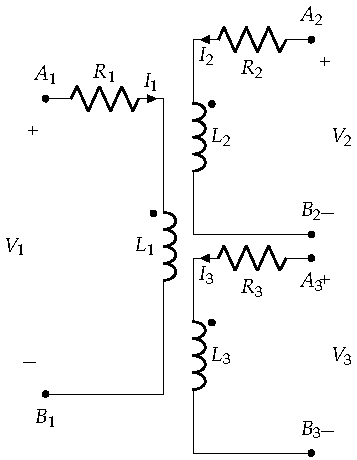
\includegraphics[height=0.5\textheight]{../figs/TrafoVariosDevanados.pdf}
% \end{center}

% \begin{align*}
%   \overline{U}_1 &= (R_1 + j \omega L_1) \cdot \overline{I}_1 + j \omega M_{12} \cdot\overline{I}_2 + j \omega M_{13} \cdot\overline{I}_3\\
%   \overline{U}_2 &= j \omega M_{12} \cdot \overline{I}_1 + (R_2 + j \omega L_2) \cdot \overline{I}_2 + j \omega M_{23} \cdot \overline{I}_3\\
%   \overline{U}_3 &= j \omega M_{13} \cdot \overline{I}_1 + j \omega M_{12} \cdot\overline{I}_2 + (R_3 + j \omega L_3) \cdot \overline{I}_3
% \end{align*}
% \end{frame}

% \begin{frame}[label={sec:org3799b6e}]{Transformador Perfecto}
% \begin{columns}
% \begin{column}{0.6\columnwidth}
% \begin{center}
% 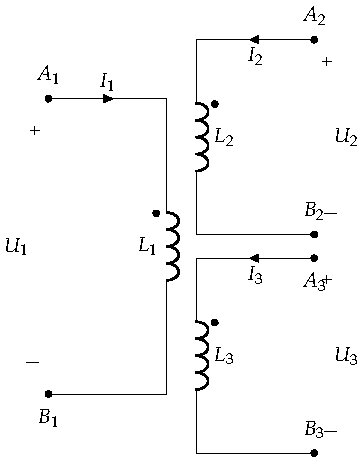
\includegraphics[height=0.8\textheight]{../figs/TrafoPerfectoVariosDevanados.pdf}
% \end{center}
% \end{column}

% \begin{column}{0.4\columnwidth}
% Las pérdidas resistivas son despreciables.
% \[
%   R_1 = R_2 = R_3 = 0
% \]

% El acoplamiento es perfecto.
% \[
%   k_{12} = k_{13} = k_{23} = 1
% \]
% \end{column}
% \end{columns}
% \end{frame}

% \begin{frame}[label={sec:orge5dab44}]{Ecuaciones del Transformador Perfecto}
% \begin{center}
% 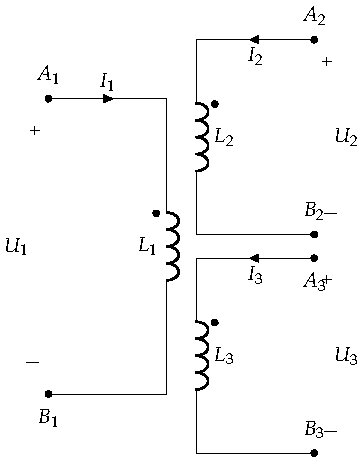
\includegraphics[height=0.5\textheight]{../figs/TrafoPerfectoVariosDevanados.pdf}
% \end{center}

% \begin{align*}
%   \overline{U}_1 &= j \omega L_1 \cdot \overline{I}_1 + j \omega M_{12} \cdot\overline{I}_2 + j \omega M_{13} \cdot\overline{I}_3\\
%   \overline{U}_2 &= j \omega M_{12} \cdot \overline{I}_1 + j \omega L_2 \cdot \overline{I}_2 + j \omega M_{23} \cdot \overline{I}_3\\
%   \overline{U}_3 &= j \omega M_{13} \cdot \overline{I}_1 + j \omega M_{12} \cdot\overline{I}_2 + j \omega L_3 \cdot \overline{I}_3
% \end{align*}
% \end{frame}

% \begin{frame}[label={sec:org7f5efb9}]{Relaciones de Transformación}
% \begin{columns}
% \begin{column}{0.6\columnwidth}
% \begin{center}
% 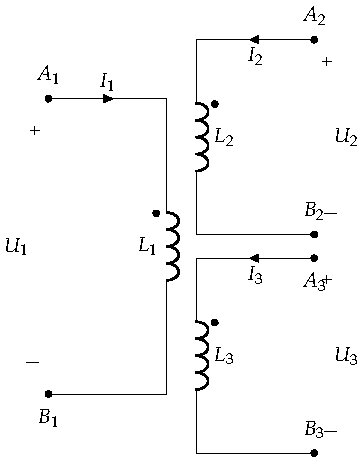
\includegraphics[height=0.6\textheight]{../figs/TrafoPerfectoVariosDevanados.pdf}
% \end{center}
% \end{column}

% \begin{column}{0.4\columnwidth}
% \begin{align*}
%   \frac{L_1}{L_2} &= \left(\frac{N_1}{N_2}\right)^2 = a^2_{12}\\
%   \frac{L_1}{L_3} &= \left(\frac{N_1}{N_3}\right)^2 = a^2_{13}
% \end{align*}

% \begin{align*}
%   \frac{\overline{U}_1}{\overline{U}_2} &= a_{12}\\
%   \frac{\overline{U}_1}{\overline{U}_3} &= a_{13}
% \end{align*}
% \end{column}
% \end{columns}
% \end{frame}

% \begin{frame}[label={sec:org271de00}]{Transformador Ideal}
% \begin{center}
% 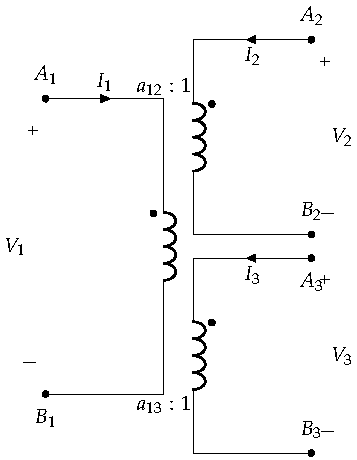
\includegraphics[height=0.9\textheight]{../figs/TrafoIdealVariosDevanados.pdf}
% \end{center}
% \end{frame}

% \begin{frame}[label={sec:org04a7201}]{Relación de Transformación del Transformador Ideal}
% \begin{center}
% 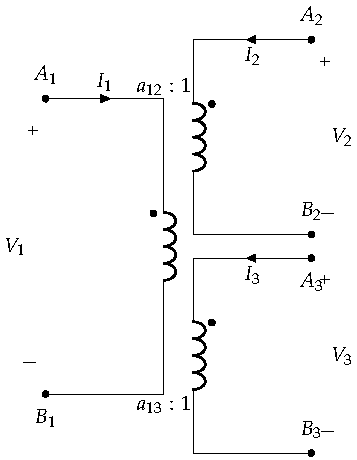
\includegraphics[height=0.35\textheight]{../figs/TrafoIdealVariosDevanados.pdf}
% \end{center}

% Debido a las condiciones de idealidad:

% \[
%   \overline{\phi}_{11} \pm \overline{\phi}_{22} \pm \overline{\phi}_{33} = 0
% \]

% \[
%   N_1 \overline{I}_1 \pm N_ 2\overline{I}_2 \pm N_3 \overline{I}_{3} = 0
% \]

% En términos de corriente:
% \[
%   \boxed{\overline{I}_1 = \mp 1/a_{12} \cdot \overline{I}_2 \mp 1/a_{13} \cdot  \overline{I}_3}
% \]
% \end{frame}

% \begin{frame}[label={sec:orgeb1473f}]{Impedancia de Entrada}
% \begin{center}
% 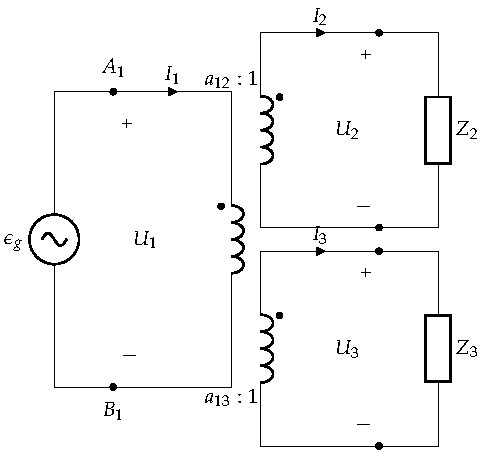
\includegraphics[height=0.9\textheight]{../figs/TrafoIdealVariosDevanados_Impedancia.pdf}
% \end{center}
% \end{frame}


% \begin{frame}[label={sec:orgef1200c}]{Impedancia de Entrada}
% \begin{columns}
% \begin{column}{0.4\columnwidth}
% \begin{center}
% 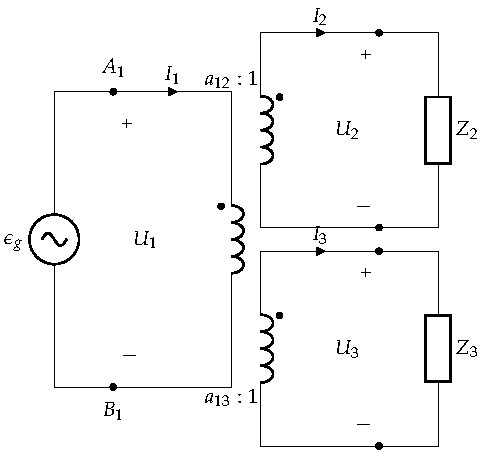
\includegraphics[height=.2\textheight]{../figs/TrafoIdealVariosDevanados_Impedancia.pdf}
% \end{center}
% \end{column}

% \begin{column}{0.6\columnwidth}
% Ecuaciones del transformador:
% \begin{align*}
%   \overline{U}_1 &= \overline{U}_2 \cdot a_{12}\\
%   \overline{U}_1 &= \overline{U}_3 \cdot a_{13}\\
%   \overline{I}_1 &= 1/a_{12} \cdot \overline{I}_2 + 1/a_{13} \cdot  \overline{I}_3
% \end{align*}

% Ecuaciones Terminales
% \begin{align*}
%   \overline{U}_2 &= \overline{Z}_2 \cdot \overline{I}_2\\
%   \overline{U}_3 &= \overline{Z}_3 \cdot \overline{I}_3
% \end{align*}

% Resultado:
% \[
%   \frac{\overline{I}_1}{\overline{U}_1} = \boxed{\overline{Y}_{in} = \frac{1}{a^2_{12} \overline{Z}_2} +  \frac{1}{a^2_{13} \overline{Z}_3}}
% \]
% \end{column}
% \end{columns}
% \end{frame}

% \begin{frame}[label={sec:orgb82f528}]{Circuito Equivalente}
% \begin{columns}
% \begin{column}{0.5\columnwidth}
% \begin{center}
% 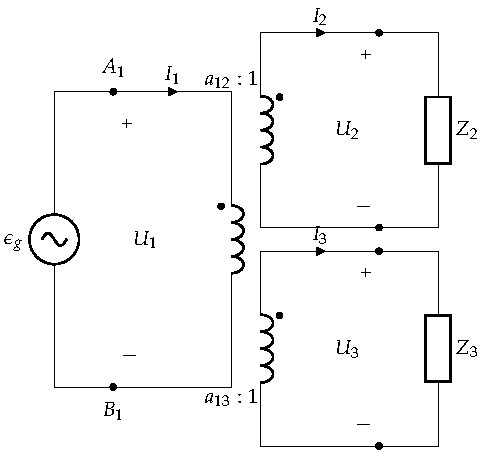
\includegraphics[height=.2\textheight]{../figs/TrafoIdealVariosDevanados_Impedancia.pdf}
% \end{center}
% \end{column}

% \begin{column}{0.5\columnwidth}
% \begin{center}
% 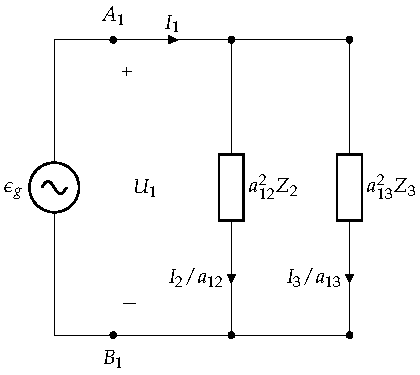
\includegraphics[height=.2\textheight]{../figs/TrafoIdealVariosDevanados_Impedancia_Equivalente.pdf}
% \end{center}
% \end{column}
% \end{columns}
% \end{frame}


% \begin{frame}[label={sec:org0ee8de8}]{Circuito Equivalente de un Transformador Perfecto}
% \begin{columns}
% \begin{column}{0.5\columnwidth}
% \begin{center}
% 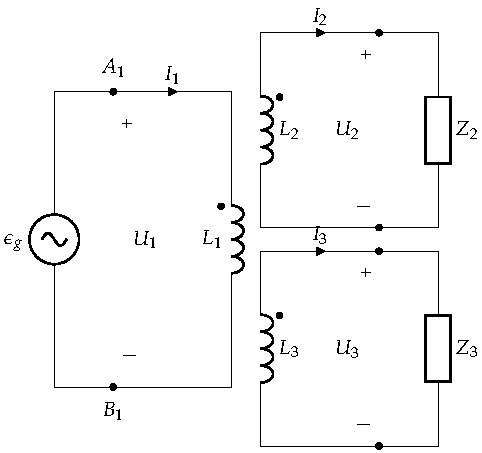
\includegraphics[width=\textwidth]{../figs/TrafoPerfectoVariosDevanados_Impedancia.pdf}
% \end{center}
% Transformador Perfecto
% \end{column}
% \begin{column}{0.5\columnwidth}
% \begin{center}
% 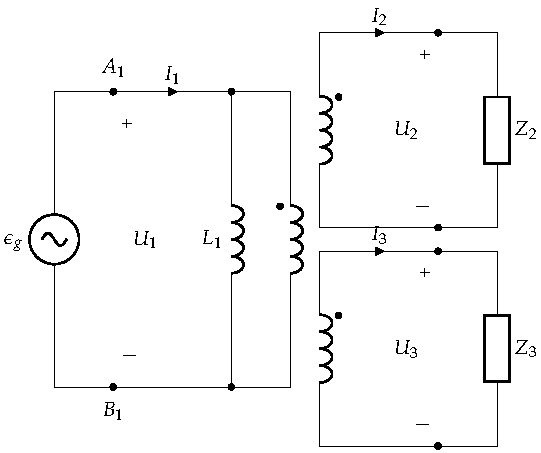
\includegraphics[width=\textwidth]{../figs/TrafoPerfectoIdealVariosDevanados_Impedancia.pdf}
% \end{center}
% Equivalente Ideal
% \end{column}
% \end{columns}
% \end{frame}

% \begin{frame}[label={sec:orgd865c57}]{Circuito Equivalente de un Transformador Perfecto}
% \begin{columns}
% \begin{column}{0.5\columnwidth}
% \begin{center}
% 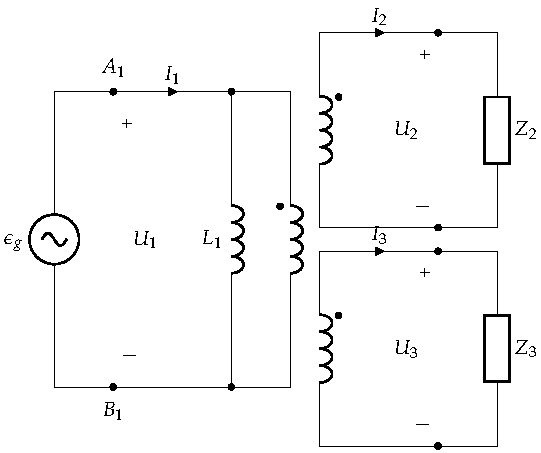
\includegraphics[width=\textwidth]{../figs/TrafoPerfectoIdealVariosDevanados_Impedancia.pdf}
% \end{center}
% \end{column}

% \begin{column}{0.5\columnwidth}
% \begin{center}
% 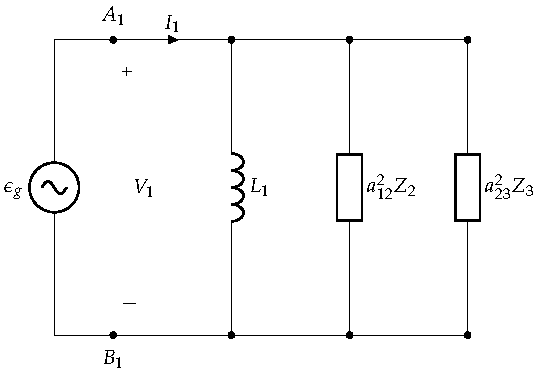
\includegraphics[width=\textwidth]{../figs/TrafoPerfectoVariosDevanados_Impedancia_Equivalente.pdf}
% \end{center}
% \end{column}
% \end{columns}
% \end{frame}
% \section{Autotransformador}
% \label{sec:org5dd3c66}
% \begin{frame}[label={sec:org962763f}]{Autotransformador Perfecto}
% \begin{center}
% 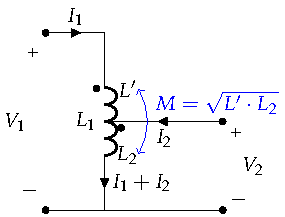
\includegraphics[height=0.9\textheight]{../figs/AutotrafoPerfecto.pdf}
% \end{center}
% \end{frame}

% \begin{frame}[label={sec:org4f6aa8f}]{Ecuaciones del Autotransformador Perfecto}
% \begin{center}
% 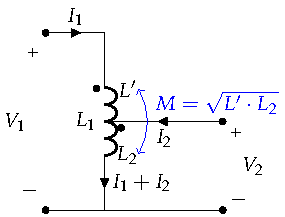
\includegraphics[height=0.5\textheight]{../figs/AutotrafoPerfecto.pdf}
% \end{center}

% \begin{align*}
%   \overline{U}_1 &= j \omega L_1 \cdot \overline{I}_1 + j \omega (M + L_2) \cdot \overline{I}_2\\
%   \overline{U}_2 &= j \omega (M + L_2) \cdot \overline{I}_1 + j \omega L_2 \cdot \overline{I}_2
% \end{align*}
% \end{frame}
% \begin{frame}[label={sec:org5642b2f}]{Circuito Alternativo del Autotransformador Perfecto}
% \begin{center}
% 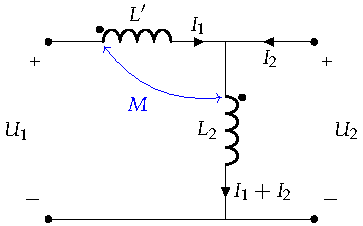
\includegraphics[height=0.8\textheight]{../figs/AutotrafoPerfecto2.pdf}
% \end{center}
% \end{frame}

% \begin{frame}[label={sec:org8075218}]{Ecuaciones del Circuito Alternativo}
% \begin{center}
% 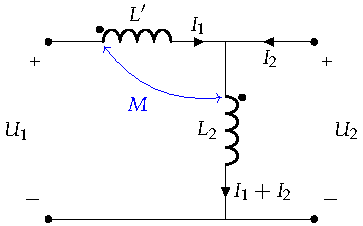
\includegraphics[height=0.5\textheight]{../figs/AutotrafoPerfecto2.pdf}
% \end{center}
% \begin{align*}
%   \overline{U}_1 &= j \omega (L' + L_2 + 2M) \cdot \overline{I}_1 + j \omega (L_2 + M) \cdot \overline{I}_2\\
%   \overline{U}_2 &= j \omega (L_2 + M) \cdot \overline{I}_1 + j \omega L_2 \cdot \overline{I}_2
% \end{align*}
% \end{frame}

% \begin{frame}[label={sec:org5055ac6}]{Ecuaciones Comparadas}
% \begin{columns}
% \begin{column}{0.4\columnwidth}
% \begin{center}
% \includegraphics[height=0.4\textheight]{../figs/AutotrafoPerfecto.pdf}
% \end{center}
% \end{column}

% \begin{column}{0.6\columnwidth}
% \begin{center}
% \includegraphics[height=0.4\textheight]{../figs/AutotrafoPerfecto2.pdf}
% \end{center}
% \end{column}
% \end{columns}

% \begin{align*}
%   \overline{U}_1 &= j \omega{\color{blue} L_1} \cdot \overline{I}_1 + j \omega{\color{red} (M + L_2)} \cdot \overline{I}_2 = j \omega{\color{blue} (L' + L_2 + 2M)} \cdot \overline{I}_1 + j \omega{\color{red} (M + L_2)} \cdot \overline{I}_2\\
%   \overline{U}_2 &= j \omega{\color{red} (L_2 + M)} \cdot \overline{I}_1 + j \omega{\color{PineGreen} L_2} \cdot \overline{I}_2 = j \omega{\color{red} (L_2 + M)} \cdot \overline{I}_1 + j \omega{\color{PineGreen} L_2} \cdot \overline{I}_2
% \end{align*}

% \begin{align*}
%   L_1 &= L' + L_2 + 2M\\
%   M' &= M + L_2
% \end{align*}
% \end{frame}

% \begin{frame}[label={sec:org63af0d4}]{Transformador Perfecto Equivalente}
% \begin{center}
% \includegraphics[height=0.5\textheight]{../figs/AutoTrafo_TrafoPerfecto.pdf}
% \end{center}

% \begin{align*}
%   L_1 &= L' + L_2 + 2M\\
%   M &= \sqrt{L' \cdot L_2}\\
%   M' &= M + L_2
% \end{align*}
% \end{frame}
% \begin{frame}[label={sec:org3722de7}]{Transformador Perfecto Equivalente}
% \begin{center}
% \includegraphics[height=0.35\textheight]{../figs/AutoTrafo_TrafoPerfecto.pdf}
% \end{center}
% Comprobamos:
% \begin{align*}
%   M' &= \sqrt{L_1 \cdot L_2} = \\
%      &= \sqrt{(L' + L_2 + 2M) L_2} =\\
%      &= \sqrt{L'L_2 + L_2^2 + 2ML_2} =\\
%      &= \sqrt{M^2 + L_2^2 + 2ML_2} = \\
%      &= M + L_2
% \end{align*}
% \end{frame}
% \begin{frame}[label={sec:org5f441d1}]{Autotransformador Ideal}
% \begin{columns}
% \begin{column}[b]{0.5\columnwidth}
% \begin{center}
% \includegraphics[height=.2\textheight]{../figs/AutoTrafoIdeal.pdf}
% \end{center}
% \end{column}
% \begin{column}[b]{0.5\columnwidth}
% \begin{center}
% \includegraphics[height=.2\textheight]{../figs/Trafo_Ideal.pdf}
% \end{center}
% \end{column}
% \end{columns}
% \end{frame} 	

%%% Local Variables:
%%% mode: latex
%%% TeX-master: "TC"
%%% ispell-local-dictionary: "castellano"
%%% End:
